
\chapter{Background Information}

This chapter describes key concepts of data provenance, IoT characterstics, and provenance models. It outlines differences that exists between provenance and log and procenance and metadata. 

\section{Data Provenance}

The oxford English dictionary defines provenance as the place of origin or earliest known history of something. An example of provenance can be seen with a college transcript. A transcript can be defined as the provenance of a college degree because it outlines all of the courses satisfied in order to attain the degree.
\par In the field of computing, data provenance also known as data lineage can be defined as the history of all transformations performed on a data object from the its creation to its current state. Cheney et al decribes provenance as the origin and history of data from its lifecycle. Buneman et al describes provenance froma database perspective as the rigin of data snd the steps in which it is derived in the database system. data provenance has immense applications and been explored in the areas of scientific computing to track how an experiments are produced for reproducability, in buisness to determine the workflow of  a process, in field of computer security for forensic analysis and intrusion detection. Provenance denotes the who, where and why of data.An example of provenance for a software systems is a web server's log file. This file contains metadata for various request and response time and ip addresses of all host systems that requests information from the server.Provenance data is represented as an acyclic graph which denotes casual relationship and dependencies between entities.Provenance ensures trust and integrity of data. The information in which provenance offers can be used in digital forensics to investigate the cause of a malicious attack and also in intrusion detection systems to further enhance the security of computing devices. 




 
\section{Internet of Things(IoT)}
There is no standard definition for IoT, however researchers have tried to define the concept of connected "things". The concept of IoT was proposed by Mark Weiser in the early 1990.  IoT represents a way in which physical objects can be linked to the digital world.



We define the internet of things(IoT) as a network of heterogeneous devices communicating together thereby making the device smarter. The notion of internet of things has been attributed to smart devices. It is believed that the interconnectivity between various hetrogenous devices allows for devices to share information in a new way. This notion of smart devices can be seen in various commercial applications such as smartwatches to smart themostasts that automatically regulates the temperature of a room. The ubiquitous nature of these devices make them ideal choices to be included in consumer products.With the recent data explosion due to the large influx in amounts of interconnected devices,information is disseminated at vast rate and with this increase bring about security and privacy issues. \\

Creating a provenance aware system is beneficial to IoT because it ensures the trust and  integrity of device. Enabling IoT device provenance aware allows devices to capture information such as the who, where and how transformations occur on a data object which enables  backtracking in an event of a malicious attack.We take a holistic aproach to provenance collection by looking at how provenance information is collected accress the IoT architectural framework from bottom(sensor layer) to the top(cloud layer).

  \textcolor{red}{TODO: Create transition from Data provenance to IoT...}   This increases productivity and also machine to machine communication.
  
  
  Due to moores law devices are getting cheaper and more technologies incoporated into consumer devices.
  
  
  
  
  
 
  
  
  \subsection{IoT Architecture}

IoT architecture consists of four distinct layers, sensor layer, device layer, gateway layer and cloud layer. The base of the architectural stack consist of sensors and actuators which collect information from IoT devices and interacts with the device layer. The device layer consists of devices(e.g mobile phones, laptops, smart devices) which are responsible for aggregating data collected from sensors and actuators. These device in turn forwards the aggregated data to the gateway layer.The gateway layer is concerned with the routing and forwarding of data collected. It could also serve as a medium of temporal storage and processing of information. This layer serves as the intermediary between the device and the cloud layer. The cloud layer is involved with the storage and processing of data collected from the gateway layer. This information can be further analyzed with advanced analytics to derive insights from the data received.  Figure 2 displays the IoT architectural stack and the interactions between the respective  layers. The resource constraints(memory , computation) decreases as you go up the architectural stack with the cloud layer having the most resource and the sensor layer having the least amount of resources


\begin{figure}[h!]
\begin{center}

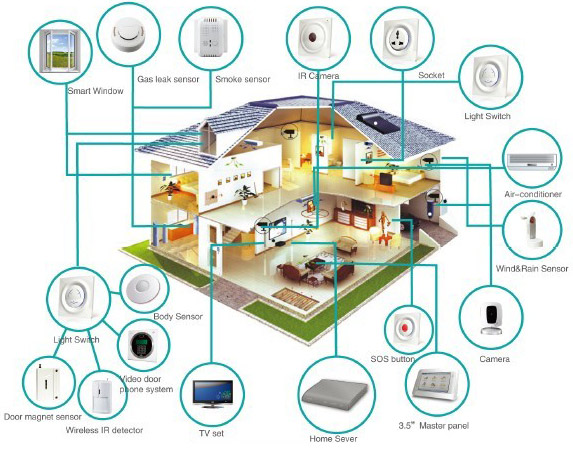
\includegraphics[height=3in]{smarthome-diagram.png}
\end{center}
\caption{Place holder for IoT Architecture Diagram}

\end{figure}



\section{Provenance and Metadata}
Metadata and provenance are often considered related but yet subtle differences exist between them. Metadata contains descriptive information about data. Metadata can be considered as provenance when there exists relationship between objects and explains how objects are . For example a web server can have metadata information such as the host and destination IP addresses which might not be considered as provenance information for a specific application.It could also contain timestamps with location of IP addresses which can be considered as provenance information. In summary metadata and provennace are not completely not the same, however an ovelap exists. Metadata contains valuable  provenance information but not all provenance information is metadata. 


\textcolor{red}{Metadata is used to represent properties of objects. Many of those properties have to do with provenance, so the two are often equated. How does metadata relate to provenance?
Descriptive metadata only becomes part of provenance when one also specifies its relationship to deriving an object. For example, a file can have a metadata property that states its size, which is not considered provenance information since it does not relate to how it was created. The same file can have metadata regarding creation date, which would be considered provenance-relevant metadata. So even though a lot of metadata has to do with provenance, both terms are not equivalent. In summary, provenance is often represented as metadata, but not all metadata is necessarily provenance.}


\section{Provenance and Log data}
Log data contains information about the activity of an object in a operating system or process.Provenance is a specialized form of Log data. It contains information specific to an application domain. Log files might contain unrealted information such as error messages, warnings which might not be considered as provenance data. Logging is limited, lacking information that shows the internal state of an object. Provenance allows for a specified collection of information that relates to the change the internal state of an object.

\section{Model for representing provenance for IoT}

In order to ensure that we properly represent and convey the right kind of provenance information in the IoT architecture, we need to satisfy the who, where, how, and what of data transformations.Provenance data is represented using a provenance model, PROV\-DM which is represented in serialized format as a JSON object. This model displays the causality and relationships of all of the data objects contained in the IoT architectural stackThis model contains information such as sensor readings, device name, and device information. This information is mapped into an appropriate provenance data model  to allow for interoperability and visualization. Provenance is represents causal dependencies between data objects. There are two models for representing provenance. These models have been applied in various literature and is considered a standard for representing provenance. Some of the models for representing provenance data are outlined below:

\subsection{Open Provenance Model(OPM)}

Open provenance model is a specification that was derived as a result of a meeting at the International Provenance and Annotation Workshop (IPAW) workshop in May 2006. OPM was created to address the need of allowing a unified way of representing provenance data amongst various applications. It allows for interchangeability between various provenance models that might exist. The goal of OPM is to develop a digital representation of provenance for entities regardless of if it is produced by a computer system or not. 

An example of such is depicted in Figure 7. This OPM graphs represents a process of driving a car.  \textcolor{red}{TODO: work on OPM Example}



OPM is represented as a directed acyclic graph which denotes causal dependency between entities. The edges in the graph denotes dependencies with its source denoting effect and its destination denoting cause.The definitions of the edges and their relationships are denoted below: 


\begin{itemize}
\item wasGeneratedBy: Shows relationship in which an entity(e,g artifact) is utilized by one or  more entities(e.g process). An entity can use multiple enities so it is important to define the role.  
\item wasControlledBy: This denotes a relationship in which an entity caused the creation of another entity.
\item used(Role): Denotes an entity requires the services of another entity in order to execute.
\item wasTriggeredBy: This relationship represents a process that was triggered by another process
\item wasDerrivedFrom: This relationship indicates that the source needs to have been generated before the destination is generated.
\end{itemize}

 There are three entities contained in the OPM model: artifact, process, agent. 

\begin{itemize}
\item
artifact: This represents the state of an entity.An artifact is graphically represented by a circle.

\item
Process: A process is an event which is taking place.A process is represented by a square object.

\item 
Agent: Agents are actors that facilitate the execution of a process.An agent is represented by a hexagon in an OPM graph.
\end{itemize}

OPM denotes all previous and current actions that have been performed on an entity and  the relationship between each entities contained in the graph. Figure 2 represents an example of an OPM acyclic graph with all of its causal dependencies. The goal of OPM is to be able to model the state of how things both digital or physical are at a given state.   

\begin{figure}[h]
\begin{center}

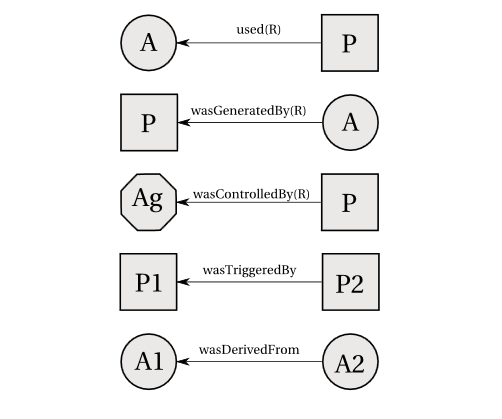
\includegraphics{opm_convention.PNG}
\end{center}
\caption{Edges and entities in OPM}
\label{autom}
\end{figure}

%\begin {center}
%\begin {tikzpicture}[-latex ,auto ,node distance =4 cm and 5cm ,on grid ,
%semithick ,
%state/.style ={ circle ,top color =white , bottom color = processblue!20 ,
%draw,processblue , text=blue , minimum width =1 cm}]
%\node[state] (C)
%{$1$};
%\node[state] (A) [above left=of C] {$0$};
%\node[state] (B) [above right =of C] {$2$};
%\path (A) edge [loop left] node[left] {$1/4$} (A);
%\path (C) edge [bend left =25] node[below =0.15 cm] {$1/2$} (A);
%\path (A) edge [bend right = -15] node[below =0.15 cm] {$1/2$} (C);
%\path (A) edge [bend left =25] node[above] {$1/4$} (B);
%\path (B) edge [bend left =15] node[below =0.15 cm] {$1/2$} (A);
%\path (C) edge [bend left =15] node[below =0.15 cm] {$1/2$} (B);
%\path (B) edge [bend right = -25] node[below =0.15 cm] {$1/2$} (C);
%\end{tikzpicture}
%\end{center}

\subsection{Provenance Data Model(Prov-DM)}

PROV-DM is a W3C standardized extension of OPM. Prov-DM is a model that is used for depict causal relationship between entities, activities and , and agents(digital or physical).  It creates a common model that allows for interchange of provenance information between heterogeneous devices. It contains two major components: types and relations. Figure below shows an example of a causal relationship between an entity, agent, and activity in a PROV-DM

%\begin{figure}[h]
%\begin{center}
%
%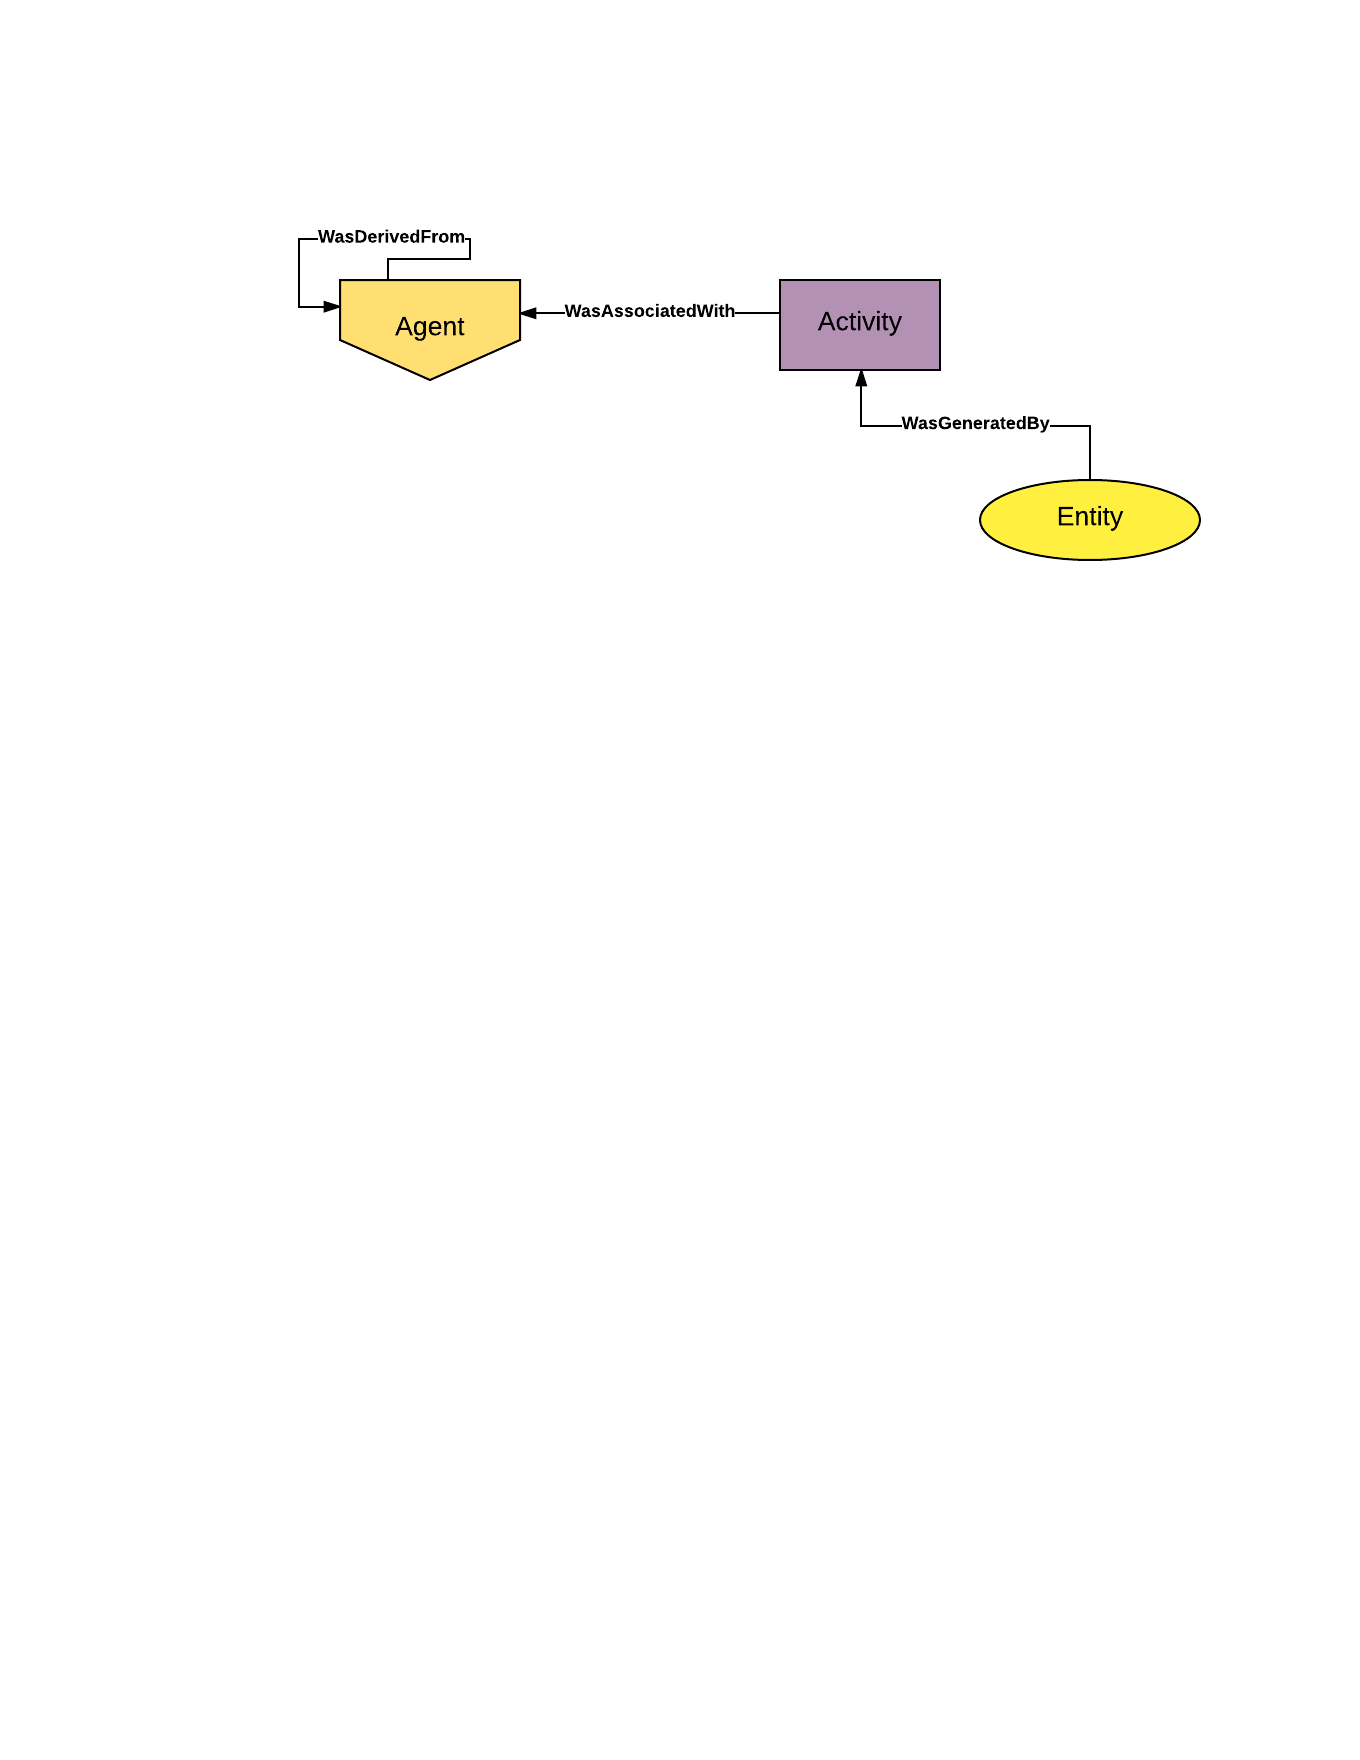
\includegraphics[height=7in]{prov_dm.PNG}
%\end{center}
%\caption{Prov DM}
%\label{autom}
%\end{figure}
%
\begin{itemize}

\item entity: An entity is a physical or digital object. An example of an entity is a file system, a process, or an motor vehicle.

\item Activity: An activity represents some form of action that occurs over a time frame.Actions are acted upon by an entity. an example of an activity is a process opening a file directory, Accessing a remote server.

\item Agent: An agent is a thing that takes ownership of an entity, or performs an activity. An example of an agent is a person, a software product, a process.
\end{itemize}

PROV-DM relations represents causal dependencies which denotes relationship between the core types(entity, activity, agent).Entities, activities and agent are represented by oval, rectangle and hexagonal shape respectively.The names of relations make use of past tense to denote past occurrence of provenance information. provenance does not keep track/estimate of future events. PROV relations are outlined below:


\begin{itemize}
\item wasGeneratedBy: This relation signifies the creation of an entity by an activity. 

\item used: This relation denotes that the functionality of an entity has been adopted by an activity.

\item wasInformedBy: This relation denotes an causality that follows the exchange of two activities.

\item wasDerievedFrom This relation represents a copy of information from an entity. 

\item wasAttributedTo: This denotes relational dependency to an agent. It is used to denote relationship between entity and agent when the activity that created the agent is unknown.

\item wasAssociatedWith:This relation denotes a direct association to an agent for an activity that occurs.This indicates that an agent plays a role in the creation or modification of the activity.

\item ActedOnBehalfOf: This denotes assigning authority to perform a particular responsibility to an agent. This could be by itself or to another agent.



\end{itemize}

Prov-DM contains similar yet subtle differences between OPM.Some of the difference between OPM and PROV-DM are described below:

\begin{itemize}

\item the main components Artifact, Process and Agent in the OPM model are changed to Entity, Action, and Agent. 

\item additional causal dependencies such as wasAttributedTo and actedOnBelafOf are included to represent direct and indirect causal dependencies respectively between agents and entities.

\end{itemize}

Since PROV-DM is built on OPM and contains easy to understand constructs of entities, we choose to use this instead of OPM. 

\subsection{PROV-JSON}

PROV-JSON is a W3C specification for relaying PROV-DM specification in JSON(Javascript Object Notation) format. It contains all of the components and relationships contained in PROV-DM. It ensures interoperability between applications using PROV-DM. It also allows for easy serialization and deserialization of PROV\-DM mappings.JSON is lightweight, easy to parse, and allows an easy way of manipulating data programmatically. An example of PROV-JSON format is described below:

\begin{figure}[h]
\begin{center}

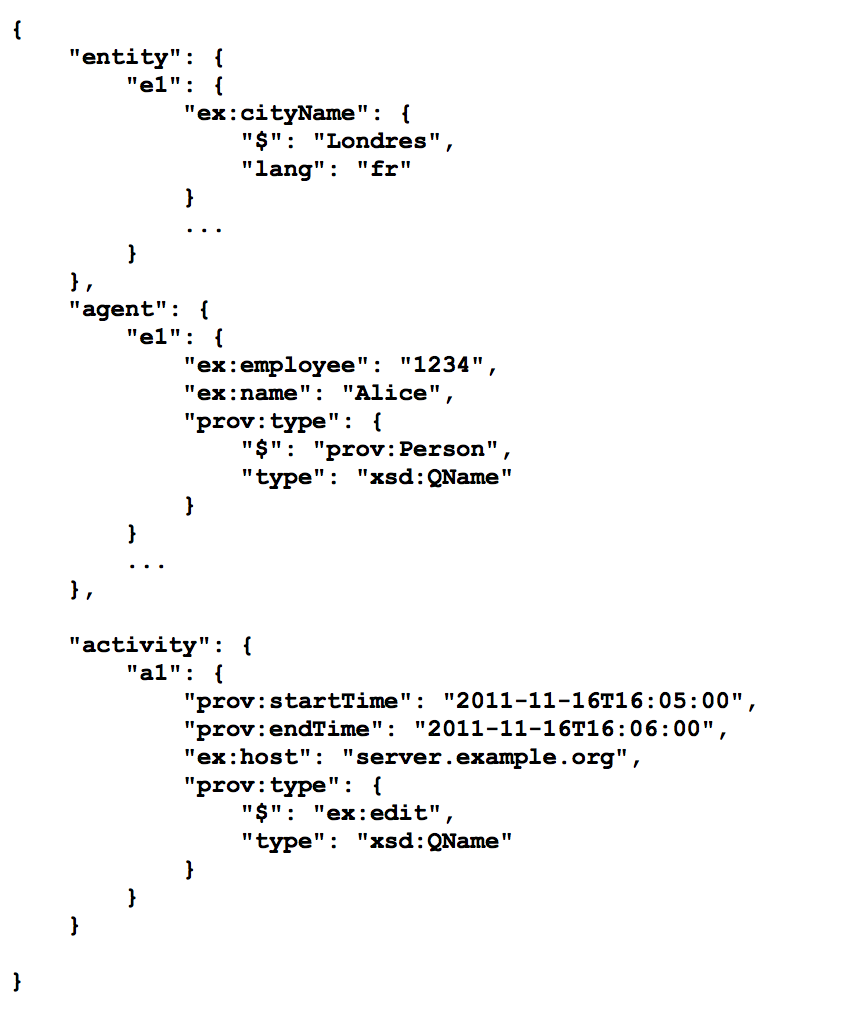
\includegraphics[height=5in]{prov_json.png}
\end{center}
\caption{PROV-JSON MODEL}

\end{figure}



\section{Overview of Relevant Compression techniques}


\subsection{Graph Compression}

\subsection{Lossy Compression}

Lossy compression is a form of data compression in which the original data can be reconstructed with some tolerance of loosing some information contained in the original data. This enables higher compression ration than lossless compression techniques.Lossy Compression is mostly used in applications that does not have strict requirements as to loosing some information. An example of a lossless compression application can be seen in image compression software where the quality of the image is not seen by the naked eye. It is also used in speech transmission. 

\subsection{Lossless Compression}
Lossless compression is a data compression technique in which the original data is reconstructed without loss of any information from. It can be used by applications which requires that the data compressed and the original data be identical. An example of such an application that requires lossless compression is text compression.  Any compression that alters the structure of the original text results to a different meaning of the text. For instance, the sentence "I have a black cat" would have a different meaning if any information is lost from it.



\subsubsection{Arithmetic Coding}

Arithmetic coding is a form of lossless compression which encodes a stream of characters into a variable size interval between [0,1). A probability is assigned to each characters contained in the string. A cumulative probability is used to calculate the interval for the respective character.The more frequent characters are encoded with shorter codes than the less frequent characters. 

\subsubsection{Dictionary Coding}



\subsubsection{Pruning Technique} 